\documentclass[a4paper,twoside]{article}
\usepackage{blindtext}  
\usepackage{geometry}

% Chinese support
\usepackage[UTF8, scheme = plain]{ctex}

% Page margin layout
\geometry{left=2.3cm,right=2cm,top=2.5cm,bottom=2.0cm}


\usepackage{listings}
\usepackage{xcolor}
\usepackage{geometry}
\usepackage{amsmath}
\usepackage{float}
\usepackage{hyperref}

\usepackage{graphics}
\usepackage{graphicx}
\usepackage{subfigure}
\usepackage{epsfig}
\usepackage{float}

\usepackage{algorithm}
\usepackage[noend]{algpseudocode}

\usepackage{booktabs}
\usepackage{threeparttable}
\usepackage{longtable}
\usepackage{listings}

% cite package, to clean up citations in the main text. Do not remove.
\usepackage{cite}

\usepackage{color,xcolor}

%% The amssymb package provides various useful mathematical symbols
\usepackage{amssymb}
%% The amsthm package provides extended theorem environments
\usepackage{amsthm}
\usepackage{amsfonts}
\usepackage{enumerate}
\usepackage{enumitem}
\usepackage{listings}

\usepackage{indentfirst}
\setlength{\parindent}{2em} % Make two letter space in the first paragraph
\usepackage{setspace}
\linespread{1.5} % Line spacing setting
\usepackage{siunitx}
\setlength{\parskip}{0.5em} % Paragraph spacing setting

% \usepackage[contents =22920202204622, scale = 10, color = black, angle = 50, opacity = .10]{background}

\renewcommand{\figurename}{图}
\renewcommand{\lstlistingname}{代码} 
\renewcommand{\tablename}{表格}
\renewcommand{\contentsname}{目录}
\floatname{algorithm}{算法}

\graphicspath{ {images/} }

%%%%%%%%%%%%%
\newcommand{\StudentNumber}{22920202204622}  % Fill your student number here
\newcommand{\StudentName}{熊恪峥}  % Replace your name here
\newcommand{\PaperTitle}{作业(一) \ 实现C-Means算法}  % Change your paper title here
\newcommand{\PaperType}{模式识别} % Replace the type of your report here
\newcommand{\Date}{2022年2月28日}
\newcommand{\College}{信息学院}
\newcommand{\CourseName}{模式识别}
%%%%%%%%%%%%%

%% Page header and footer setting
\usepackage{fancyhdr}
\usepackage{lastpage}
\pagestyle{fancy}
\fancyhf{}
% This requires the document to be twoside
\fancyhead[LO]{\texttt{\StudentName }}
\fancyhead[LE]{\texttt{\StudentNumber}}
\fancyhead[C]{\texttt{\PaperTitle }}
\fancyhead[R]{\texttt{第{\thepage}页,共\pageref*{LastPage}页}}


\title{\PaperTitle}
\author{\StudentName}
\date{\Date}

\lstset{
	basicstyle          =   \sffamily,          % 基本代码风格
	keywordstyle        =   \bfseries,          % 关键字风格
	commentstyle        =   \rmfamily\itshape,  % 注释的风格,斜体
	stringstyle         =   \ttfamily,  % 字符串风格
	flexiblecolumns,                % 别问为什么,加上这个
	numbers             =   left,   % 行号的位置在左边
	showspaces          =   false,  % 是否显示空格,显示了有点乱,所以不现实了
	numberstyle         =   \zihao{-5}\ttfamily,    % 行号的样式,小五号,tt等宽字体
	showstringspaces    =   false,
	captionpos          =   t,      % 这段代码的名字所呈现的位置,t指的是top上面
	frame               =   lrtb,   % 显示边框
}

\lstdefinestyle{PythonStyle}{
	language        =   Python, % 语言选Python
	basicstyle      =   \zihao{-5}\ttfamily,
	numberstyle     =   \zihao{-5}\ttfamily,
	keywordstyle    =   \color{blue},
	keywordstyle    =   [2] \color{teal},
	stringstyle     =   \color{magenta},
	commentstyle    =   \color{red}\ttfamily,
	breaklines      =   true,   % 自动换行,建议不要写太长的行
	columns         =   fixed,  % 如果不加这一句,字间距就不固定,很丑,必须加
	basewidth       =   0.5em,
}

\begin{document}
	
%%%%%%%%%%%%%%%%%%%%%%%%%%%%%%%%%%%%%%%%%%%%
\makeatletter % change default title style
\renewcommand*\maketitle{%
	\begin{center} 
		\bfseries  % title 
		{\LARGE \@title \par}  % LARGE typesetting
		\vskip 1em  %  margin 1em
		{\global\let\author\@empty}  % no author information
		{\global\let\date\@empty}  % no date
		\thispagestyle{empty}   %  empty page style
	\end{center}%
	\setcounter{footnote}{0}%
}
\makeatother
%%%%%%%%%%%%%%%%%%%%%%%%%%%%%%%%%%%%%%%%%%%%
	
	
\thispagestyle{empty}

\vspace*{1cm}

\begin{figure}[h]
	\centering
	
\includegraphics[width=4.0cm]{logo.png}
\end{figure}

\vspace*{1cm}

\begin{center}
	\Huge{\textbf{\PaperType}}
	
	\Large{\PaperTitle}
\end{center}

\vspace*{1cm}

\begin{table}[h]
	\centering	
	\begin{Large}
		\renewcommand{\arraystretch}{1.5}
		\begin{tabular}{p{3cm} p{5cm}<{\centering}}
			姓\qquad 名 & \StudentName  \\
			\hline
			学\qquad号 & \StudentNumber \\
			\hline
			日\qquad期 & \Date  \\
			\hline
			学\qquad院 & \College  \\
			\hline
			课程名称 & \CourseName  \\
			\hline
		\end{tabular}
	\end{Large}
\end{table}

\newpage

\title{
	\Large{\textcolor{black}{\PaperTitle}}
}
	
	
\maketitle
	
\tableofcontents
 
\newpage
\begin{spacing}{1.2}
	
\section{实现和运行结果}

\subsection{选择特征和实现}

首先做出Iris数据集两两变量的散点图和单个变量的分布曲线图,如图\ref{Fig.pairplot}(见\nameref{sec:appA}),可以发现萼片长款参数单独出现对聚类结果没有较好的贡献,重合部分较多。为了充分利用数据,再计算萼片面积和花瓣面积。发现组合“花瓣面积-萼片面积”、“花瓣面积-萼片长度”等都有较好的区分,但是\textbf{考虑到K-Means算法团块状聚类的特点},我选择做出散点图最符合团状特点的“花瓣面积-萼片面积”作为用于聚类的两个特征,但是该特征选择依然难以避免iris-virginica和iris-versicolor两类有所重叠。实现见\nameref{sec:appB}中的代码\ref{code:kmeans}。

该实现使用了以下第三方库:

\begin{itemize}
	\item \textbf{Pandas} 用于读取CSV数据集文件、计算平均数和方差等统计量
	\item \textbf{NumPy} 用于加速数值计算
\end{itemize}

\subsection{运行结果}

聚类结果如图\ref{Fig.result},图上除了聚类结果还显示了初始时选择的点、聚类中心。可见C-Means给出了较好的聚类结果。

\begin{figure}[h] 
	\centering
	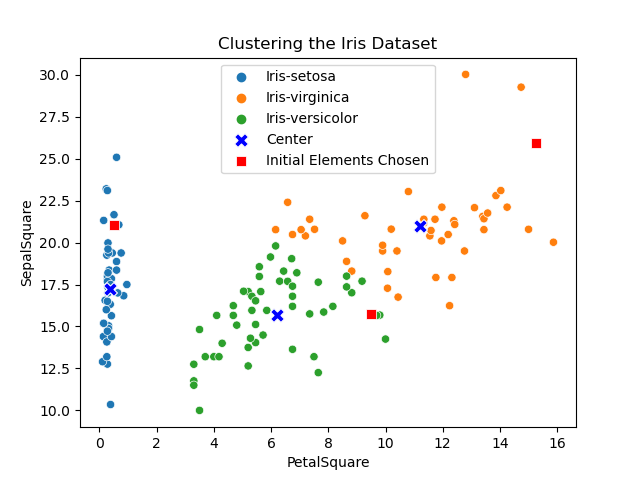
\includegraphics[width=0.5\textwidth]{../result.png} 
	\caption{聚类结果可视化}
	\label{Fig.result}
\end{figure}

\section{误差统计和分析}

\begin{figure}[h] 
	\centering
	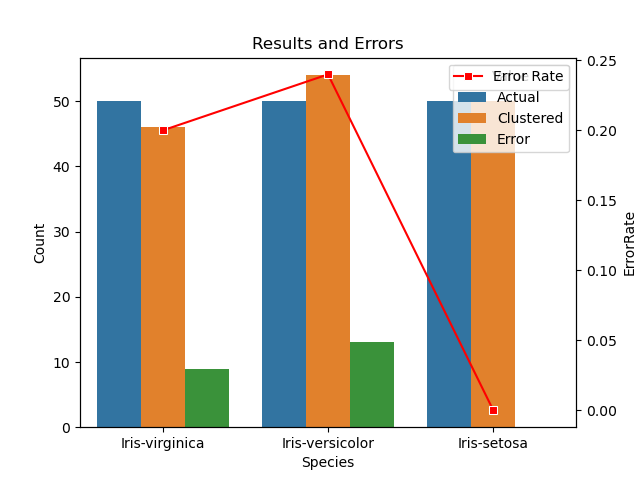
\includegraphics[width=0.5\textwidth]{../errors.png} 
	\caption{结果和错误统计}
	\label{Fig.error}
\end{figure}

\begin{table}[h]
	\caption{误差统计}
	\label{tbl:sta}
	\begin{center}
		\begin{tabular}{ccccc}
			\toprule  
			物种& 数量& 聚类数量 &错误量 &错误率\\
			\midrule 
			Iris-virginica& 50& 46 & 9 &0.2\\
			Iris-versicolor& 50& 54 & 13 & 0.24\\
			Iris-setosa&50 &50 &0 &0 \\
			\bottomrule 
		\end{tabular}
	\end{center}
\end{table}


为了进一步判断聚类的效果,将聚类结果和Iris数据集中的标签对照,统计类的大小、错误量、错误率,得到表\ref{tbl:sta}和图\ref{Fig.error}。可以发现C-Means较好地区分出了iris-setosa,但是iris-virginica和iris-versicolor中存在一定的错误,这和选择特征时的观察相符合,即iris-virginica和iris-versicolor的分布有重合的部分。

但是,考虑到错误率相当低,可以认为C-Means算法给出了很好的聚类效果。


\appendix

\section{附录: Iris数据集多变量图}
\label{sec:appA}

\begin{figure}[H] 
	\centering
	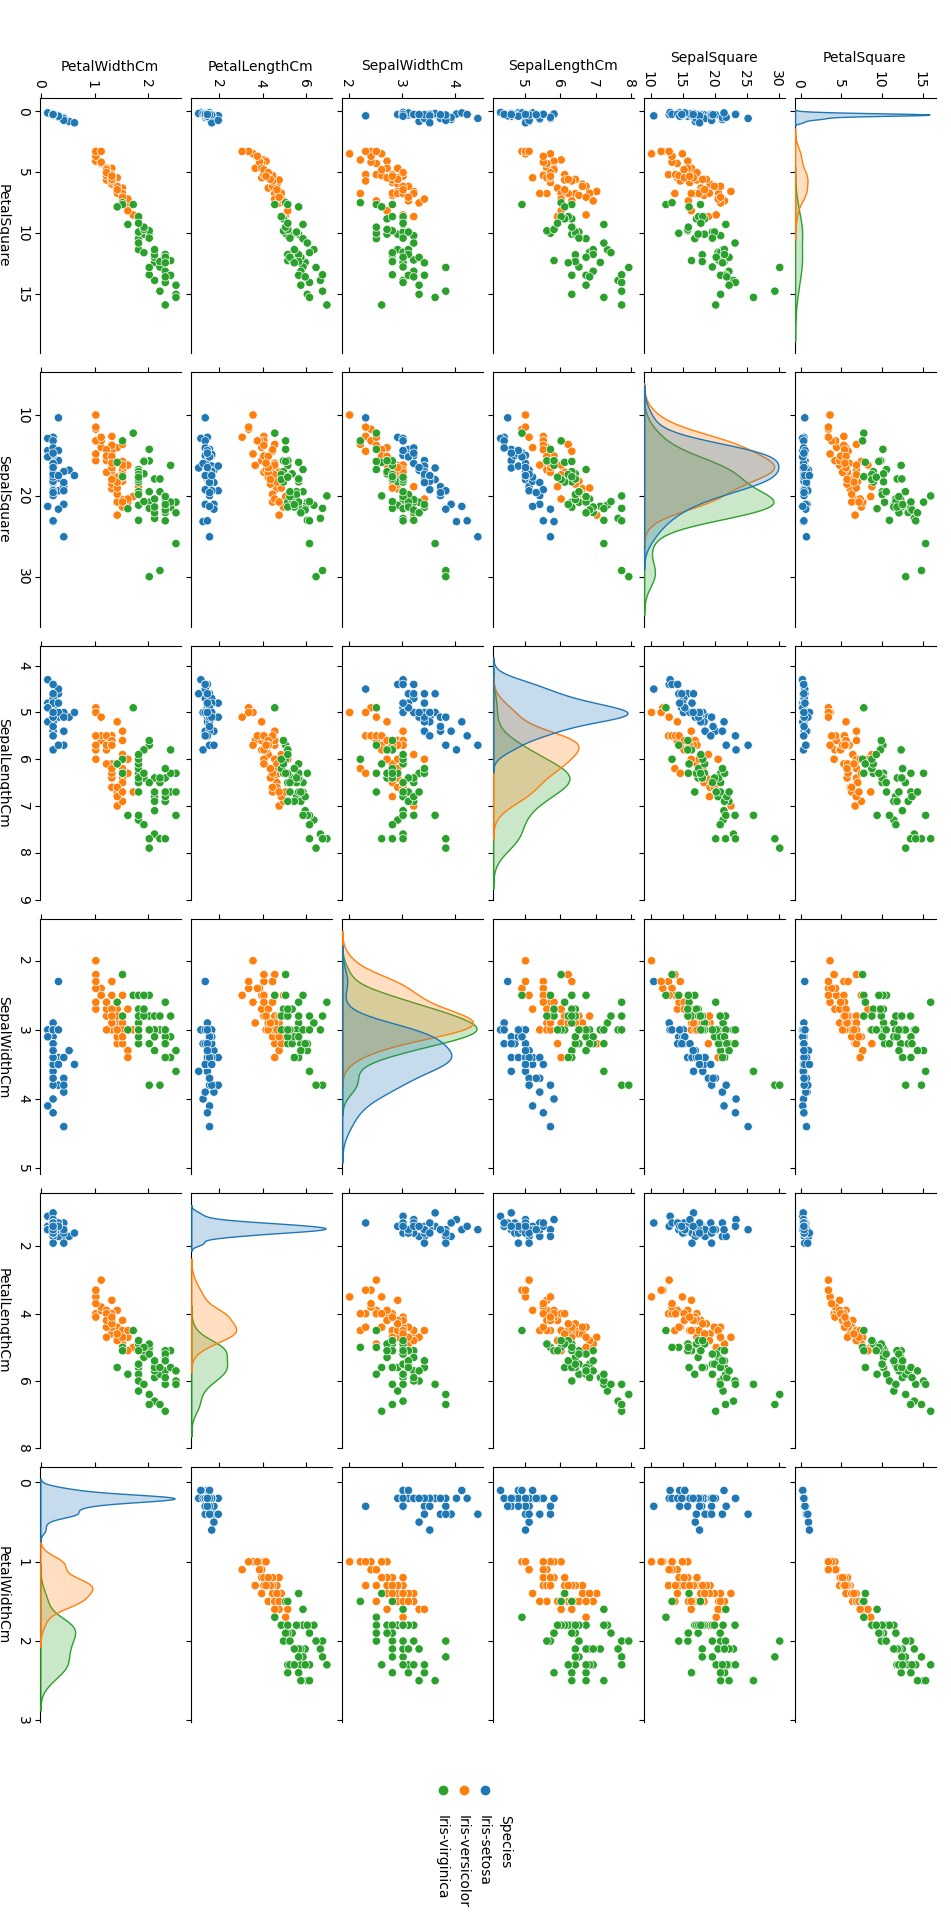
\includegraphics[width=0.7\textwidth]{../pairplot.png} 
	\caption{Iris数据集多变量图(Pair Plot)}
	\label{Fig.pairplot}
\end{figure}

\section{附录: 核心部分源代码}
\label{sec:appB}

\begin{lstlisting}[language=Python,numbers=left,style=PythonStyle,caption=瑞利分布生成,label={code:kmeans}]
class KMeans:
	def __init__(self, feats: pd.DataFrame, k: int):
		self.tries = 0
		self.feats = feats
		self.k = k
	
	def _wcss(self, centroids, cluster) -> float:
		ret = 0.0
		for i, val in enumerate(self.feats.values):
		ret += np.sqrt(
		(centroids[int(cluster[i]), 0] - val[0]) ** 2 + (centroids[int(cluster[i]), 1] - val[1]) ** 2)
		return ret
	
	def cluster(self, max_tries: int = 32767):
		self.tries = 0
		
		cluster = np.zeros(self.feats.shape[0])
		
		centroid_indexes, centroids = self.feats.sample(n=self.k).index, self.feats.sample(n=self.k).values
		
		while self.tries < max_tries:
			self.tries += 1
			
			for id, row in enumerate(self.feats.values):
				min_dist = float('inf')
				for cid, centroid in enumerate(centroids):
					dist = np.sqrt((centroid[0] - row[0]) ** 2 + (centroid[1] - row[1]) ** 2)
					if dist < min_dist:
						min_dist, cluster[id] = dist, cid
					clustered_centroids = self.feats.copy().groupby(by=cluster).mean().values
					if np.count_nonzero(centroids - clustered_centroids) == 0:
						break
					else:
						centroids = clustered_centroids
		return centroid_indexes, centroids, cluster, self._wcss(centroids, cluster)
	
	def get_tries(self) -> int:
		return self.tries

\end{lstlisting}

\end{spacing}
\end{document}